% c04 ------ 源文件 QuantumWorkTry.tex 第 1480--1986 行
% 所属章节：第 3 节 实费米子（Real Fermions），含 3.1--3.7 各小节与图 9
% 说明：本文件只含正文片段（UTF-8，无导言区）；公式、编号、引用与原文逐字一致，译者批注以 LaTeX 注释形式附于相应段落前后。

\section{实费米子（Real Fermions）}\label{realf}

\begin{keytakeaways}
\begin{itemize}[leftmargin=1.6em,itemsep=0.2em,topsep=0.2em]
  \item \textbf{物理图像}：本节讨论欧氏号差下边界模为实费米子的拓扑物态，基本例子是二加一维时间反演不变拓扑超导体，其次是二加一维拓扑绝缘体；前者边缘是只与引力耦合的马约拉纳费米子，后者边缘是带电荷的狄拉克费米子，但其电荷与时间反演对易。
  \item \textbf{数学工具}：反对称双线性型的普法夫量、狄拉克算子的模 2 指标、谱流与映射环面、pin 结构、配边不变性、APS 边界条件与泡利--维拉尔斯正规化。
  \item \textbf{核心结论}：实费米子的谱只有本征值的正负配对，可以存在未配对零模，其数目模 2 即模 2 指标；该指标是配边不变量，从而给出三维流形上配分函数符号由模 2 指标决定的自旋拓扑量子场论；体理论必须与边界马约拉纳费米子合并才在物理上自洽，此即反常流入。
\end{itemize}
\end{keytakeaways}

本节讨论这样一类拓扑物态：在欧氏号差下，其边界模是实费米子。我们的基本例子将是 $2+1$ 维 $\sT$-不变拓扑超导体。不过，我们也会讨论 $2+1$ 维拓扑绝缘体。

\subsection{谱的对称性（Symmetry Of The Spectrum）}\label{rsf}

在两个时空维数中，我们只需要两个伽马矩阵。在欧氏号差下，它们应当满足 $\{\g_a,\g_b\}=2\delta_{ab}$，并且可以取为 $2\times 2$ 实矩阵，例如 $\g_1=\sigma_1$、$\g_2=\sigma_3$。

% [Tutor Note: 原文第 1492--1493 行取 $\g_a$ 为实矩阵，故 $\slashed{D}=\sum_i\g^i D_i$ 为实反对称；由此 $\D=\i\slashed{D}$ 为纯虚且反对称，又因 $(iA)^\dagger=-iA^T=iA$（$A^T=-A$）而自动厄米。原文同处 “on on unorientable 2-manifold” 重出一词，应为 “on an unorientable 2-manifold”（源第 1493 行）。]

因此，算子 $\slashed{D}=\sum_{i=1}^2 \gamma^i D_i$ 是实反对称算子。相应的厄米狄拉克算子 $\D=\i\slashed{D}$ 是虚的、反对称的。即便在不可定向的二维流形上，这也成立。

考虑此情形下的本征值问题 $\D\chi=\lambda\chi$。谱在 $\lambda\to -\lambda$ 下不变，因为若 $\D\chi=\lambda\chi$，则 $\D\chi^*=-\lambda\chi^*$。注意我们利用了一个反线性操作 $\T:\chi\to\chi^*$，它满足 $\T^2=1$。相反，对赝实费米子，我们在第 \ref{topsup} 节为证明谱对每个 $\lambda$ 值都加倍，用的是满足 $\T^2=-1$ 的反线性对称性。在实情形下，对称性 $\lambda\to-\lambda$ 把 $\lambda\not=0$ 的本征值配对，但可能存在未配对的零模。（实际上，这些零模会表示一个模 2 指标，我们将在第 \ref{inter} 节讨论。）目前我们假定一般情形下没有零模。

% [Tutor Note: 关键在于实表示下的反线性操作 $\T:\chi\to\chi^*$ 满足 $\T^2=1$，只给出 $\lambda\leftrightarrow-\lambda$ 的配对；赝实表示下 $\T^2=-1$ 且与狄拉克算子对易，才导致每个本征值的二重简并（Kramers 型简并，参看第 \ref{inter} 节对三维可定向流形的论证以及附录 \ref{twod} 中的 $\T'$）。实情形下零模不被对称性排除，这正是模 2 指标得以存在的原因。]

$2+1$ 维 $\sT$-不变拓扑超导体的边缘模是一个 $1+1$ 维马约拉纳费米子（只与引力耦合）。这里没有 $\U(1)$ 对称性，费米路径积分最好理解为反对称双线性型 $\DD$ 的普法夫量。用厄米狄拉克算子 $\D$ 定义 $\DD$ 的方式，与第 \ref{topsup} 节讨论的赝实费米子略有不同。彼时取 $\DD_{\gamma\beta}=\veps_{\gamma\alpha}\D^\alpha_\beta$，其中 $\veps_{\alpha\beta}$ 是费米子场空间中的不变反对称张量；现在则取 $\DD_{\gamma\beta}=\delta_{\gamma\alpha}\D^\alpha_\beta$，其中 $\delta_{\gamma\alpha}$ 是不变对称张量。

由此得到的结果是：$\DD$ 是 $2\times 2$ 分块的直和，$\D$ 的每一对本征值 $\lambda_i,-\lambda_i$ 对应一个这样的分块：
\be\label{molfo}\DD=\bigoplus_i \bp 0&\lambda_i\cr -\lambda_i & 0 \ep. \ee
这与赝实情形形成对照：在那种情形下，$\DD$ 对每一对具有{\it 相同}本征值 $\lambda$ 的态有一个 $2\times 2$ 分块。

% [Tutor Note: 由分块形式可得 $\det\DD=\prod_i(-\lambda_i^2)$，而 $\Pf(\DD)=\pm\prod_i\lambda_i$；因此 $\Pf(\DD)^2=\det\DD$。这就是实反对称双线性型上“普法夫量平方等于行列式”的论证，也是 $\Pf(\DD)$ 的符号只能定义到整体正负号为止的根源。]

一个重要的细节是：给定反对称双线性型 $\DD$ 后，其“斜本征值” $\lambda_i$ 只在相差一个符号的意义下唯一确定。在第 $i$ 个分块上作用 $2\times 2$ 矩阵 $\mathrm{diag}(1,-1)$ 所给出的正交变换，会把式（\ref{molfo}）中 $\lambda_i$ 的符号反转。因此，{\it 在相差一个符号的意义下}（并且模去正规化的需要），费米路径积分为
\be\label{wolfo}\Pf(\DD)=\prod_i\lambda_i.\ee

% [Tutor Note: 在第 $i$ 分块上取正交变换 $\diag(1,-1)$ 会使 $\lambda_i\to-\lambda_i$，同时因该变换行列式为 $-1$ 而使 $\Pf(\DD)$ 变号。故“斜本征值”只在相差符号的意义下确定；要真正定义路径积分还须正规化（泡利--维拉尔斯），原文括注 “modulo the need for regularization” 即指此。]

宽泛地说，我们处在一个熟悉的情形中。要确定 $\Pfaff(\DD)$ 的符号，我们需要知道，在模 2 意义下，有多少个 $\lambda_i$ 应当被视为负的。一般而言，这样的问题没有自然的答案。然而我们注意到，作为二维流形 $Y$ 的度规张量 $g$ 的函数，$\Pfaff(\DD)$ 应当在每一对本征值 $\lambda_i,-\lambda_i$ 穿过 0 时变号。因此为了得到部分答案，我们可以先在二维流形 $Y$ 上选定某个度规 $g_0$，取定 $\Pfaff(\DD)$ 的符号，然后通过数出从 $g_0$ 到 $g$ 的插值过程中本征值对穿过 0 的次数，来确定符号作为 $g$ 的函数。

\begin{figure}[htbp]
  \centering
  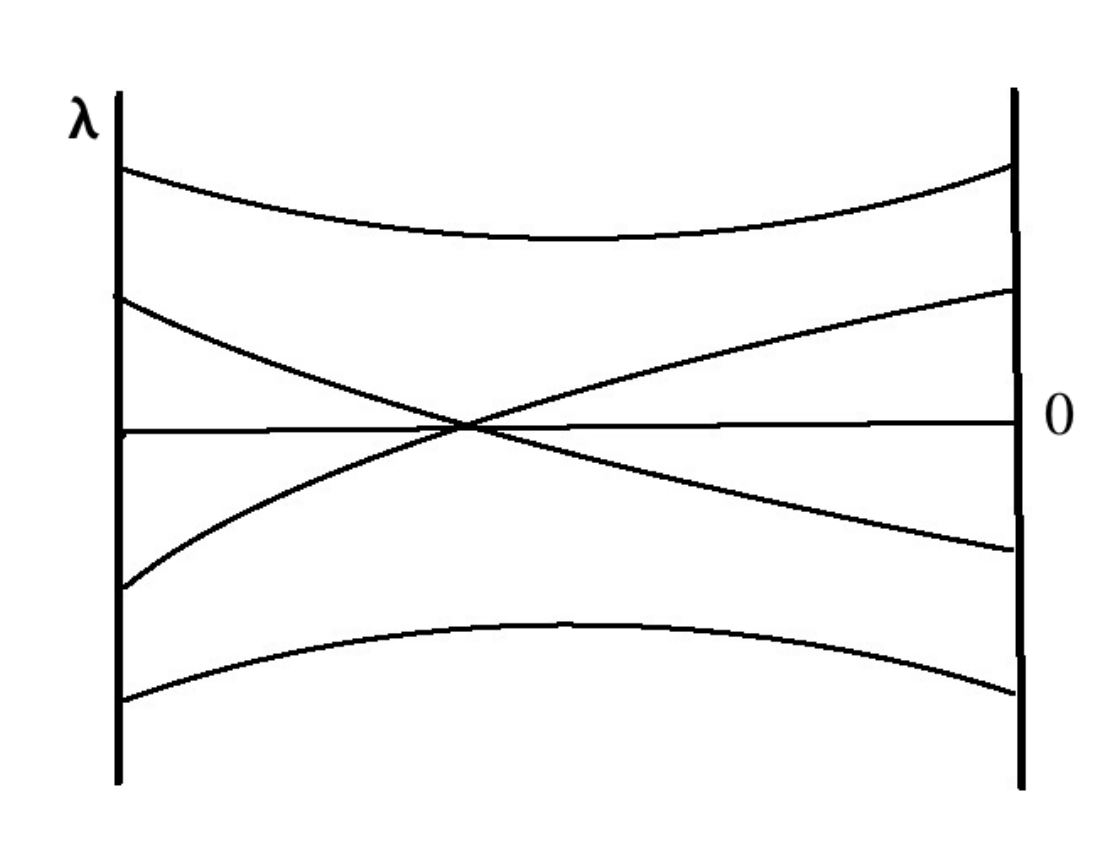
\includegraphics[width=0.55\textwidth]{fig09.png}
  \caption{实费米子的谱流。谱在 $\lambda\leftrightarrow-\lambda$ 下对称。每当一对本征值流经 0，费米路径积分就改变符号，因此我们按模 2 计算：从初始度规 $g_0$ 插值到它在某个微分同胚 $\phi$ 下的像 $g_0^\phi$ 的过程中，此事发生了多少次。在图中所示的例子里，它发生了一次，故 $\Pfaff(\DD)$ 在 $\phi$ 下为奇。（原文第 44 页，图 9）}
  \label{real}
\end{figure}

为了理解 $\Pfaff(\DD)$ 在微分同胚 $\phi$ 下的行为，我们必须按模 2 计算：当通过由 $s\in[0,1]$ 参数化的一族度规 $g_s$，从初始度规 $g_0$ 插值到它在 $\phi$ 下的共轭 $g_0^\phi$ 时，$\Pfaff(\DD)$ 的符号改变了多少次（图 \ref{real}）。与图 \ref{flow} 的赝实情形的差别在于：那里数的是当 $s$ 从 0 增到 1 时本征值（或本征值对）从 $\lambda<0$ 到 $\lambda>0$ 的净流动，这是一个整数值不变量；现在我们关心的是按模 2 数出一对本征值 $\pm\lambda$ 穿过 0 的次数。容易看出，这只是一个模 2 拓扑不变量。

% [Tutor Note: 此处“仅为模 2”的原因：每有一对 $\pm\lambda$ 穿过 0，$\Pf(\DD)$ 就变号一次；净穿行次数是整数，但符号只记录其奇偶。与赝实情形的整数值谱流不同，这里没有典范的定向区分正、负穿行方向，故不变量只能取 $\Z_2$ 值；这也正是映射环面上模 2 指标的定义方式。]

在第 \ref{pseudo} 节中，我们利用了如下事实：赝实费米子在 $d$ 个时空维数中产生的整数值谱流不变量，可用 $D=d+1$ 维中狄拉克算子的指标来表达。不假定 $\U(1)$ 对称性的最一般形式见式（\ref{neft}）。实费米子的 $\Z_2$ 值谱流不变量同样是某种狄拉克指标，只是不那么熟悉。它等于 $D$ 维中狄拉克算子的模 2 指标 \cite{AStwo}，我们将之记作 $\zeta$。这是一个相当微妙的不变量。在关于费米路径积分整体反常的早期论文 \cite{Witold,Witoldtwo} 中已经证明：$d$ 个时空维数中实费米子的模 2 谱流不变量，等于 $D=d+1$ 维中相应的模 2 狄拉克指标 $\zeta$。于是费米路径积分的变换律为
\be\label{zott}\Pf(\DD)\to \Pf(\DD)(-1)^\zeta, \ee
其中 $\zeta$ 是映射环面上狄拉克算子的模 2 指标。其证明与式（\ref{worf}）、（\ref{neft}）的证明类似；我们记得，那两式反映的是 $d$ 个时空维数中赝实费米子的谱流与 $D=d+1$ 维中普通狄拉克指标之间的关系 \cite{APS,DCG,Kiskis}。

% [Tutor Note: 式（\ref{zott}）中的 $\zeta$ 是映射环面上的模 2 指标，等于 $d$ 维实费米子谱流不变量的模 2 值。证明与式（\ref{worf}）、（\ref{neft}）平行，都归结为把 APS 指标定理用于 $D=d+1$ 维（参看 \cite{APS,DCG,Kiskis}）；由于普通指标在奇数维恒为零，这里必须用 Atiyah--Singer 指标定理的模 2 版本 \cite{AStwo}，而不能用积分公式。]

\subsection{关于模 2 指标的插叙（An Interlude On The Mod 2 Index）}\label{inter}

从物理上定义模 2 指标最直接的方式，就是注意到以下事实。一般地，假设在 $D$ 个时空维数中，我们可以为某个费米子系统写出作用量：
\be\label{facte}I=\int\d^Dx \bar\psi\DD\psi. \ee
$\DD$ 唯一普遍的性质是它可以被看作反对称双线性型------反对称来自费米统计。反对称双线性型 $\DD$ 的典范形式是若干 $2\times 2$ 分块与一些零本征值的直和：
\be\label{conform}\bp 0&a_1& && && \cr
                                   -a_1 & 0 &&&& \cr
                                    && 0 & a_2 &&&\cr
                                     && -a_2&0 &&&\cr
                                     &&&& \ddots && \cr
                                     &&&&&0 & \cr
                                      &&&&&&0 \ep. \ee
$\DD$ 的零模数目是模 2 意义下的拓扑不变量，因为当人们改变出现在非零分块中的参数 $a_1,a_2,\dots$ 时，零模只能成对地出现或消失。零模数目 mod 2 称为模 2 指标。（作为这一定义的例子，读者可以看出：若 $\Omega$ 是有限维向量空间 $V$ 上的反对称双线性型，则其模 2 指标就是 $V$ 的维数 mod 2。）

% [Tutor Note: 反对称矩阵经正交变换可化为这种分块标准形；当某个 $a_i\to0$ 时，对应的 $2\times 2$ 分块退化为两个零本征值，故零模只能成对出现------“零模数目的奇偶性”因此在参数变动下不变，这就是模 2 指标良定义的全部内容。注意它是 $\Z_2$ 值的不变量，而不是某个整数指标的模 2 约化。]

以下是低维模 2 指标的最简单例子。（在所有这些例子中，我们只考虑与引力耦合的费米子。）在一维情形，只有一个伽马矩阵 $\g_1$ 满足 $\g_1^2=1$，故把它表示为 $\g_1=1$，并考虑单分量费米子场 $\psi$。无边的紧致一维流形是一个圆周 $S^1$。自旋结构有两种可能，取决于 $\psi$ 服从周期还是反周期边界条件。狄拉克方程为 $\d\psi/\d t=0$，周期情形有 1 个零模，反周期情形没有。因此对周期或反周期费米子，模 2 指标分别为 1 或 0。

在二维情形，可以考虑只与引力耦合的单分量手征费米子 $\psi$（$2+1$ 维手征超导体的边缘模），它只能在{\it 可定向}二维流形上表述。紧致可定向二维流形的一个例子是环面 $T^2$，例如复 $z$ 平面对下式的商：
\be\label{zp}z\cong z+1\cong z+\i.\ee
手征费米子的狄拉克方程是 $\partial \psi/\partial \bar z=0$。自旋结构有 4 种，取决于 $\psi$ 在 $z\to z+1$ 与 $z\to z+\i$ 下是周期还是反周期。在全周期情形有 1 个零模，其余情形没有。因此模 2 指标恰在全周期自旋结构下非零。

% [Tutor Note: 这里的“标准事实”是二维磁场中狄拉克算子的零模计数（Landau 能级）：在手征性固定时，零模数目由磁通量与手征性共同决定。更一般地，二维可定向流形上正手征费米子的模 2 指标等于该自旋结构的 Arf 不变量（即 $\dim\ker\bar\partial\bmod 2$），这可由阿蒂亚--辛格指标定理得到；环面上 Arf 不变量为奇的情形正是全周期自旋结构。]

二维中的马约拉纳费米子 $\psi$ 又如何？在可定向二维流形上，$\psi$ 可分解为正手征与负手征分量 $\psi_+$ 与 $\psi_-$，而零模的狄拉克方程 $\slashed{D}\psi=0$ 分裂为 $\psi_+ $ 与 $\psi_-$ 各自的方程。$\psi_+$ 零模的复共轭是一个 $\psi_-$ 零模，故 $\psi$ 的零模数目平凡地为偶数，模 2 指标必然为零。

若把马约拉纳费米子表述在不可定向的二维流形上，情况就不是这样。作为一个具体例子，考虑克莱因瓶 KB，它由二维环面 (\ref{zp}) 对变换 $z\to \bar z+1/2$ 作商得到。等价地，置 $z=x_1+\i x_2$ 引入实坐标，则等价关系为
\be\label{rp}(x_1,x_2)\cong (x_1+1,x_2)\cong (x_1,x_2+1)\cong (x_1+1/2,-x_2).  \ee
我们通过要求下式在 KB 上定义一个 $\pin^+$ 结构\footnote{这一概念是不可定向流形上自旋结构的类比物，在附录 \ref{unor} 中有描述。}：
\be\label{tp}\psi(x_1,x_2)=\psi(x_1+1,x_2)=\psi(x_1,x_2+1)=\g_2\psi(x_1+1/2,-x_2).\ee
$\psi$ 在 $T^2$ 上本应有两个零模，其中一个是过渡到 KB 时被投影掉的；所以在这个 $\pin^+$ 结构下，$\psi$ 的模 2 指标为 1。

% [Tutor Note: $\pin^+$ 指反射在旋量上平方为 $+1$ 的结构（$\sR^2=1$），$\pin^-$ 则取 $\sR^2=-1$（见附录 \ref{unor}）。正是 $\pin^+$ 结构使整体定义的实结构 $\T=\psi\to\psi^*$（$\T^2=1$）存在，从而在任何（可定向或不可定向）二维流形上都有谱对称 $\lambda\leftrightarrow-\lambda$；可定向情形还可额外定义 $\T'=\beta\psi^*$（$\T'^2=-1$，与 $\D$ 对易），给出本征值的偶重数。变换 $z\to\bar z+1/2$ 是反转 $x_2$ 并作平移的无固定点对合；$T^2$ 上的两个马约拉纳零模在 $\g_2$ 的本征值 $\pm1$ 下各给一个组合，而投影条件 $\psi=\g_2\psi$ 只保留 $+1$ 组合，另一个被投影掉，故 KB 上恰有一个零模。]

作为最后一个例子，考虑 $D=3$ 个时空维数中的双分量马约拉纳费米子 $\psi$。这种系统有狄拉克作用量，因此可以定义模 2 指标。该模 2 指标在可定向三维流形 $X$ 上恒为零。事实上，在可定向三维流形上，狄拉克算子的本征值总具有偶数重数，这一点我们先前用式（\ref{norg}）所定义的反线性操作说明过。然而在不可定向三维流形上，模 2 指标可以非平凡。一个简单例子是 $X=\KB\times S^1$，其中 $\KB$ 及其上的自旋结构已由式（\ref{rp}）、（\ref{tp}）定义，而 $S^1$ 上取周期自旋结构。$\psi$ 唯一的零模是在 $S^1$ 方向为常数的模，其在 KB 上的限制正是上一段找到的零模。故模 2 指标为 1。

% [Tutor Note: 可定向三维流形上本征值的偶重数来自反线性操作（\ref{norg}）的 Kramers 型论证：该操作与 $\D$ 对易且平方为 $-1$，故每个本征空间是四元数向量空间，其复维数为偶。于是零模数目的奇偶性恒为 0，$\zeta=0$。在 $\KB\times S^1$ 上取周期自旋结构，沿 $S^1$ 的常数零模得以保留，故指标不为零。]

我们以下述强调来结束这段模 2 指标导引：尽管名为模 2 指标，它并不是某个普通指标乃至任何整数值不变量的模 2 约化。事实上，我们已在一维与三维给出了模 2 指标非平凡的例子，而普通指标在奇数维恒为零。阿蒂亚--辛格指标定理的模 2 版本 \cite{AStwo} 并不给出模 2 指标的公式\footnote{更确切地说，该公式用 K 理论表达模 2 指标，但并不给出通常意义下积分形式的公式。}，不像普通指标有人们熟悉的阿蒂亚--辛格指标公式。它确实蕴含模 2 指标是配边不变量，因而特别地，存在一个三维 sTQFT（定义在自旋流形或更确切地 $\pin^+$ 流形上），其配分函数为 $(-1)^\zeta$。在讨论该理论在带边流形上的情形之前，我们先停下来说明二维马约拉纳费米子整体反常的几个简单例子。

% [Tutor Note: 配边不变性给出同态 $\Omega_3^{\pin^+}\to\Z_2$，其像即 $(-1)^\zeta$；可定向（自旋）情形因 $\Omega_3^{\spin}=0$，该同态平凡，与“$X$ 可定向时理论平凡”相符。作为对照，普通狄拉克指标是四维自旋配边群 $\Omega_4^{\spin}\cong\Z$ 上的不变量（$\hA$ 的积分；第 2 节中 $(-1)^{\I/2}$ 的配边不变性即源于此）。模 2 指标不能写成这种积分公式，这正是原文强调它“不是任何整数值不变量的模 2 约化”的含义；阿蒂亚--辛格的模 2 指标定理用 KO 理论表述它。]

\subsection{整体反常的简单例子（Simple Examples Of The Global Anomaly）}\label{simpex}

我们在第 \ref{inter} 节了解到，在 $D=3$ 时狄拉克算子的模 2 指标在可定向流形上恒为零，但在不可定向流形上，只与引力耦合的马约拉纳费米子的模 2 指标可以非零。

这应当意味着：在 2 个时空维数中，马约拉纳费米子 $\psi$ 只要仅在可定向二维流形上表述、并且只允许保定向的微分同胚，就是自洽的；否则就会出现反常。

若把马约拉纳费米子 $\psi$ 表述在不可定向二维流形上，或允许反定向的对称性，则其反常可由一些初等例子看出，并不真正需要一般形式体系。首先考虑 $\psi$ 场在克莱因瓶 KB 上的情形，我们以之作为不可定向二维流形的例子。如上所述，在 KB 上取适当的 pin 结构时，模 2 指标非零。这意味着一般情形下狄拉克算子只有一个 $c$-数零模 $\chi_0$。其余模在谱的对称性 $\lambda\leftrightarrow-\lambda$ 下按自然方式配对。在这种情形下，费米路径积分中的测度在数费米子 mod 2 的对称性 $(-1)^F$ 下为奇。具体地说，KB 上的费米子配分函数因零模而为零，但（未归一化的）单点函数 $\langle \int\d^2x\sqrt g\bar\chi_0\psi\rangle$------带有移除该零模的算符插入------非零。由于这个关联函数含有奇数个费米子插入，它在 $(-1)^F$ 下为奇。

显然，不必考虑映射环面也能理解这个例子；但用映射环面构造又该如何理解它？流形 $Y$ 的任何能作用于费米子的微分同胚都可以有两种不同的作用方式，二者相差一个整体符号。特别地，$Y$ 的平凡微分同胚可以被取为对费米子平凡作用，或取为乘以 $-1$。若把 $Y$ 的平凡微分同胚提升为对费米子平凡作用，就得到平凡对称性 1；若取为对费米子作用 $-1$，就得到对称性 $(-1)^F$。因此我们可以把平凡对称性 1 或非平凡对称性 $(-1)^F$ 看作微分同胚的特殊情形，并应用映射环面构造。

与 $\KB$ 的平凡微分同胚相联系的映射环面就是乘积 $\KB\times S^1$。平凡微分同胚作用于费米子的两种提升，对应两种不同的 $\pin^+$ 结构：费米子沿 $S^1$ 方向周期或反周期。（$\KB$ 上的 $\pin^+$ 结构是任意的，在此讨论中保持固定。）平凡对称性 1 与对称性 $(-1)^F$ 分别对应反周期与周期的 $\pin^+$ 结构。这类似于统计力学中的事实：给定哈密顿量 $H$，为计算迹 $\Tr\,e^{-\beta H}$ 或 $\Tr\,(-1)^Fe^{-\beta H}$，我们在周长为 $\beta$ 的圆周上做路径积分，而费米子绕圆周分别取反周期或周期。现在用这两种 $\pin^+$ 结构计算 $\KB\times S^1$ 上的模 2 指标。若费米子在 $S^1$ 上反周期，对应平凡对称性 1，则 $\KB\times S^1$ 上狄拉克算子的最低本征值为 $\pi/\beta$（或更大），其中 $\beta$ 同样是圆周的周长。此时没有零模，故映射环面的模 2 指标为零，意味着 $\KB$ 上的路径积分测度在平凡对称性下不变。但若费米子在 $S^1$ 上周期，对应对称性 $(-1)^F$，则如第 \ref{inter} 节所见，$\KB\times S^1$ 上的模 2 指标与 $\KB$ 上的相同。这意味着，恰在 $\KB$ 上模 2 指标非零时，$\KB$ 上的路径积分测度在 $(-1)^F$ 下为奇。

% [Tutor Note: 两种提升相差整体符号，正对应统计力学中 $\Tr e^{-\beta H}$（反周期）与 $\Tr(-1)^F e^{-\beta H}$（周期）的区别；只有非平凡提升（此处为 $(-1)^F$）可能带有反常，故反周期情形的模 2 指标必为零。原文第 1692 行 “the mod 2 index of the mapping cylinder” 中的 “mapping cylinder” 应为 “mapping torus”（映射环面，即 $\KB\times S^1$）。]

在这些陈述中，$\KB$ 可以换成任意二维流形 $Y$。只要 $Y$ 上有非平凡的模 2 指标，从而 $(-1)^F$ 有反常，该反常就会出现在映射环面 $Y\times S^1$ 的模 2 指标中。

作为另一个简单例子，考虑可定向二维流形 $T^2$ 上的马约拉纳费米子 $\psi$。但这次考虑一个作为某一坐标反射的微分同胚 $\phi$，它反转 $T^2$ 的定向。在 $T^2$ 上取两个方向都周期的自旋结构，$\psi$ 有 2 个零模，记作 $\chi_1$ 与 $\chi_2$。由于这些零模，$\psi$ 场在 $T^2$ 上的配分函数为零，但（未归一化的）两点函数
\be\label{tolf}\left\langle\int_Y\d^2x \sqrt g \bar\chi_1\psi\cdot \int_Y\d^2x\sqrt g\bar\chi_2\psi\right\rangle\ee
非零。两个零模中，一个线性组合在 $\phi$ 下为偶，一个为奇，故式（\ref{tolf}）中的矩阵元在 $\phi$ 下为奇，表明路径积分测度在 $\phi$ 下为奇。

让我们再次尝试用映射环面构造理解这个整体反常。取 $T^2$ 为 $x_2-x_3$ 平面对 $(x_2,x_3)\cong (x_2+1,x_3)\cong (x_2,x_3+1)$ 的商，并假定马约拉纳费米子场 $\psi$ 在两个方向上都是周期的。考虑 $\phi$ 的作用为 $(x_2,x_3)\to (-x_2,x_3)$。为构造与 $\phi$ 相联系的映射环面，我们引入一份由另一变量 $x_1$ 参数化的 $\R$，并考虑 $\R\times T^2$ 对 $(x_1,x_2,x_3)\to (x_1+1/2,-x_2,x_3)$ 的商。但这只是构造熟悉的 3-流形 $\KB\times S^1$ 的另一种方式。我们还须说明希望 $\phi$ 如何作用于费米子。为此我们规定：$\KB\times S^1$ 上的费米子场 $\psi $ 就是 $\R\times T^2$ 上的费米子场，在 $T^2$ 方向周期，且满足 $\psi(x_1+1/2,-x_2,x_3)=\g_2\psi(x_1,x_2,x_3)$。但这就给出已在第 \ref{inter} 节考虑过的 $\KB\times S^1$ 上的 $\pin^+$ 结构。如那里所解释，该 $\pin^+$ 结构下的模 2 指标非零，故映射环面构造再次探测到 $T^2$ 反射对称性的整体反常。

\subsection{与时间反演不变拓扑超导体相联系的体 sTQFT（Bulk sTQFT Associated To the $\sT$-Invariant Topological Superconductor）}\label{bulkboundary}

现在考虑这样的 sTQFT：它在带 $\pin^+$ 结构的闭 3-流形 $X$ 上的配分函数为 $(-1)^\zeta$。若 $X$ 可定向，该理论是平凡的；但一般而言并非如此。

我们的第一个任务是解释：为什么这个 sTQFT 是 $D=3$ 个时空维数中 $\sT$-守恒拓扑超导体的体态。论证的风格应当与第 \ref{why} 节相似。

我们从洛伦兹号差出发，考虑两个三维费米子 $\psi_1$、$\psi_2$，它们在 $\sT$ 下以相反方式变换\footnote{在式（\ref{worx}）中，我们为一对三维费米子 $\psi_1$、$\psi_2$ 写了有质量的狄拉克方程，并假定它们在 $\sT$ 下以相同方式变换。然而它们是复狄拉克费米子，且式（\ref{worx}）中乘在质量项上的因子 $\i$ 是为 $\sT$-不变性所必需的。对马约拉纳费米子，狄拉克方程必须是实的，故这个 $\i$ 因子不可能出现；联系两个费米子 $\psi_1,\psi_2$ 的 $\sT$-不变质量项只在它们在 $\sT$ 下以相反符号变换时才可能存在。}：
\be\label{molf}\sT\psi_1(t,x_1,x_2)=\g_0\psi_1(-t,x_1,x_2),~~~\sT\psi_2(t,x_1,x_2)=-\g_0\psi_2(-t,x_1,x_2).\ee
选择相反符号，是为了能够有一个 $\sT$-守恒的非对角质量项 $m\bar\psi_1\psi_2$。（对角质量项 $m'\bar\psi_1\psi_1$ 或 $m''\bar\psi_2\psi_2$ 破坏 $\sT$。）拓扑平凡与拓扑非平凡绝缘体之间的相变在 $m$ 变号时发生。现在我们把该系统的配分函数作为 $m$ 的函数，在欧氏号差的紧致流形 $X$ 上研究。假设 $X$ 及其上的 $\pin^+$ 结构使得 $\zeta\not=0$。那么在 $m=0$ 时，$\psi_1$ 与 $\psi_2$ 都有奇数个零模（一般各为 1 个）。需要奇数次插入 $m\bar\psi_1\psi_2$ 才能抬升这些零模，因此配分函数正比于 $m$ 的奇次幂；于是只要 $\zeta\not=0$，它在穿过 $m=0$ 时就变号。若 $\zeta=0$ 则没有这种变号。所以若配分函数对比如 $m>0$ 为正定，则对 $m<0$ 其符号为 $(-1)^\zeta$。

更精确的解释如下。由于 $\psi_1$ 与 $\psi_2$ 在一个反定向对称性下以相反方式变换，它们合起来成为定向三维流形 $\h X$ 上的单个马约拉纳费米子 $\h\psi$，而后者是 $X$ 的定向双重覆盖。$\psi_1-\psi_2$ 系统在 $X$ 上的配分函数与 $\h \psi$ 在 $\h X$ 上的配分函数相同。为把这一配分函数说清楚，我们（与第 \ref{zelfan} 节的做法颇为类似）加入与 $\psi_1,\psi_2$ 统计相反的泡利--维拉尔斯正规化子场 $\chi_1,\chi_2$，以及一个 $\sT$-守恒质量项 $\mu\bar\chi_1\chi_2$。在 $\h X$ 上，它们合为单个正规化子场 $\h\chi$。$\h X$ 有一个反定向对称性（$\h X$ 对该对称性的商就是原来的 $X$）。$\h X$ 上的狄拉克算子与这样的对称性反对易（见关于式（\ref{refact}）的讨论），因此 $\h X$ 上狄拉克算子的非零本征值在 $\lambda\to-\lambda$ 下配对。（由于反线性对称性（\ref{norg}），$\hat X$ 上的谱对每个 $\lambda$ 值还有加倍；但如式（\ref{rf}）那样，马约拉纳费米子配分函数只取每一对中的一个本征值来计算。）设 $\h\psi$ 的质量为 $m$、$\h\chi$ 的质量为 $\mu$，则一对 $\lambda,-\lambda$ 对费米路径积分的贡献为
\be\label{zeffo}\frac{\lambda+\i m}{\lambda+\i \mu}~~\frac{-\lambda+\i m}{-\lambda+\i \mu}. \ee
这总是正的，与 $\mu$、$m$ 的符号无关，故非零模对正规化路径积分的贡献总是正的。现在假设 $X$ 上无质量狄拉克算子有 $\upiota$ 个零模（其中 $\upiota\cong\zeta$ mod 2）。那么 $\h X$ 上的场 $\h\psi$ 有 $2\upiota$ 个零模。由于一次质量插入可以抬升 $\h\psi$ 或 $\h\chi$ 的两个零模，每一对这样的零模在 $\h\psi$ 路径积分中给出因子 $m$，在正规化子路径积分中给出因子 $1/\mu$。因此路径积分正比于 $(m/\mu)^\upiota$；当 $m$ 与 $\mu$ 同号时为正定，否则其符号为 $(-1)^\zeta$。

% [Tutor Note: 乘积可写成 $\left|\lambda+\i m\right|^2/\left|\lambda+\i\mu\right|^2$，故对任意实 $\lambda$ 与任意符号的 $m,\mu$ 都为正------这就是原文 “This is always positive” 的由来。零模部分给出 $(m/\mu)^\upiota$：每一对零模在 $\h\psi$ 行列式中贡献 $m$，在正规化子行列式中贡献 $1/\mu$；因 $\upiota\cong\zeta\pmod 2$，其符号为 $(-1)^\zeta$。注意 $2\upiota$ 个零模来自 $\h X$ 是双重覆盖。]

$m$ 与 $\mu$ 同号的情形对应拓扑平凡的 $\sT$-不变超导体。拓扑非平凡的情形是 $m$ 与 $\mu$ 反号。后一情形才是拓扑上有趣的情形，而 $(-1)^\zeta$ 就是与之相联系的体 sTQFT 的配分函数。

\subsection{将 sTQFT 延拓到带边流形（Extending the sTQFT To A Manifold With Boundary）}\label{extending}

我们希望把这个 sTQFT 延拓到 $X$ 具有空间边界 $Y$ 的情形。为此，需要把模 2 指标 $\zeta$ 的定义延拓到 $X$ 有这种边界的情形。然而，不存在保持对称性的局部边界条件能够用来定义 $\zeta$。

让我们仔细考察这个关键点。若 $X$ 可定向，则其边界 $Y$ 也可定向，并且可以仿照式（\ref{torz}）为狄拉克方程定义局部边界条件。设 $\vec n$ 为 $Y$ 的单位法向量。于是我们可以施加边界条件
\begin{equation}\label{tumf}\gamma\cdot n\,\psi|_{Y}=\pm \psi|_Y,\end{equation}
（符号可作某种选择），而这就是最一般可能的协变边界条件。\footnote{局部边界条件必须在 $Y=\partial X$ 上把费米子分量的一半置零，而式（\ref{tumf}）是在 $p\in Y$ 处法平面旋转下保持不变的最一般做法。若改用任何其他矩阵代替 $\gamma\cdot n$，就会破坏局部旋转对称性。}无论取哪个符号，这都是物理上合理的经典边界条件，\footnote{量子力学上，带这种边界条件的 $D=3$ 费米子沿 $\partial X=Y$ 会有微扰引力反常 \cite{HW}。这在本题中并不重要，因为我们关心的是 $D=3$ 费米子的模 2 指标，而不是它的配分函数。}而在此边界条件下，可以定义狄拉克算子的模 2 指标。然而若 $Y$ 不可定向，该边界条件在整体上无意义。看出这一点的一个快捷方式如下。从双分量费米子场 $\psi$ 出发，边界条件（\ref{tumf}）选出沿 $Y$ 可以非零的一个分量，而不难看出\footnote{在局部欧氏标架中，可取三个伽马矩阵为 $\g_a=\sigma_a$，$a=1,\dots,3$，满足 $\g_1\g_2\g_3=\i$。设边界法向为 3 方向。沿边界的二维手征性由 $\i\g_1\g_2=-\g_3$ 度量，故对 $\slashed{n}=\g_3$ 本征值的条件（\ref{tumf}）选出一种二维手征性。}该分量具有二维意义下的确定手征性。但若 $Y$ 不可定向，手征性无法沿 $Y$ 整体定义，故边界条件（\ref{tumf}）整体上无意义。

若 $Y$ 可定向并选定一个定向，则取某种符号的边界条件（\ref{tumf}）有意义。把 $\zeta$ 定义为带某种符号选择的 $X$ 上狄拉克算子的模 2 指标，我们就可以在带边 3-流形上定义一个三维 sTQFT，其配分函数为 $(-1)^\zeta$。这给出三维 sTQFT 的一个有能隙、拓扑上无序但{\it 破坏对称性}的边界条件。说它破坏对称性，是因为式（\ref{tumf}）中符号的选择涉及一种二维手征性的选择，从而破坏沿边界的反射或时间反演对称性。

若使用整体 APS 边界条件，就可以 $\sT$-不变地定义 $\zeta$。具体而言，这相当于把 $X$ 换成图 \ref{longer} 中的非紧流形 $X'$，并把 $\zeta$ 定义为狄拉克算子{\it 平方可积}零模空间的维数 mod 2。这给出 $\zeta$ 的一个 $\sT$-不变定义，但如此定义的 $\zeta$ 不是拓扑不变量。当 $Y=\partial X$ 上的度规变化到使 $Y$ 上二维狄拉克算子的一对本征值穿过 0 时，$X$ 上的 APS 边界条件发生跳变，$\zeta$ 也随之跳变。

% [Tutor Note: 用 APS 边界条件即“在 $Y$ 上接一段无限长柱面”并取平方可积零模；当边界二维算子的本征值穿零时，APS 投影算子不连续，$\zeta$ 跳变，故它不是拓扑不变量。$(-1)^\zeta$ 的跳变恰由边界马约拉纳费米子路径积分的变号补偿，乘积 $|Z_\psi|(-1)^\zeta$ 光滑，这就是反常流入的标准机制。]

此时 $(-1)^\zeta$ 的符号发生跳变，因此在这个情形下，配分函数为 $(-1)^\zeta$ 的体理论本身在物理上不自洽。不过，到此应当已经清楚我们该怎么说。配分函数为 $(-1)^\zeta$ 的体理论必须与由边界上的马约拉纳费米子组成的边界系统合并。合并系统的配分函数为
\be\label{overdo}|Z_\psi|(-1)^\zeta.\ee
这里只要边界费米子的一对本征值 $\pm \lambda$ 穿过 $\lambda=0$，即只要预期边界费米子的路径积分会变号，$(-1)^\zeta$ 就跳变。因此乘积在物理上是自洽的。

\subsection{可定向情形与手征对称性（The Orientable Case And Chiral Symmetry）}\label{orch}

现在更仔细地考察 $Y$ 可定向的情形。此情形下，除我们稍后提及的一个限制外，可以假定 $Y$ 是可定向自旋流形 $X$ 的边界。这样的流形有 $\zeta=0$。事实上，第 \ref{inter} 节中证明 $X$ 可定向时 $\zeta=0$ 的论证，在 $\partial X\not=0$ 时只要使用 APS 边界条件仍然成立。

由于此情形下 $(-1)^\zeta$ 恒为 1，我们断定：若 $Y$ 可定向，就可以合理地定义 $Y$ 上马约拉纳费米子配分函数为正定。一个更直接的解释是：若 $Y$ 可定向，则 $Y$ 上的马约拉纳费米子 $\psi$ 可分解为正手征与负手征场 $\psi_+$ 与 $\psi_-$ 之和；而且 $\psi_+$ 与 $\psi_-$ 的作用量和路径积分互为复共轭。故整体路径积分为正。

只要 $Y$ 与 $X$ 可定向，配分函数公式（\ref{overdo}）就不依赖于 $X$------因为对任何 $X$ 都有 $\zeta=0$------因此看来我们可以忘掉 $X$，从而得到 $Y$ 上无质量马约拉纳费米子理论作为一个纯二维理论的定义。然而有一个细节需要小心。到此为止，我们只假定 $Y$ 可定向，却并未真正选定定向。马上就会看到，要给出 $Y$ 上马约拉纳费米子理论的完整定义，需要选定 $Y$ 的一个定向，从而只允许保定向的微分同胚作为对称性。这不应当令人意外，因为要分析 $Y$ 的反定向对称性，映射环面构造会要求我们考虑不可定向三维流形 $X$ 上的模 2 指标，而这可以非平凡，正如我们在第 \ref{inter} 节的例子中所讨论的。

需要小心的原因是：对给定的 $Y$ 与给定的自旋结构，合适的 $X$ 可能不存在。$X$ 存在性的障碍恰在 $Y$ 满足如下条件时出现：正手征费米子 $\psi_+$ 在 $Y$ 上的模 2 指标 $\zeta_Y$ 不为零。（由复共轭，$\zeta_Y$ 也是负手征费米子 $\psi_-$ 在 $Y$ 上的模 2 指标。）这个模 2 指标是配边不变量，故若它在 $Y$ 上非零，则带有给定自旋结构的 $Y$ 不是可定向自旋流形 $X$ 的边界。

假设这个指标在 $Y$ 上非零。则 $\psi_+$ 与 $\psi_-$ 各有奇数个零模；为简单起见，假定这个数目为 1（一般值），并把 $\psi_{+,0}$ 与 $\psi_{-,0}$ 记作 $\psi$ 的模展开中零模的系数。对 $Y$ 上非零费米子模的路径积分自然是正的，因为 $\psi_-$ 路径积分是 $\psi_+$ 路径积分的复共轭。由于 $\psi_{+,0}$ 与 $\psi_{-,0}$ 是零模的系数，在没有算符插入时它们的路径积分为零，因此我们该问的是如何定义路径积分测度。但除非选定 $Y$ 的一个定向，没有自然的方式定义该测度的符号：我们写 $\d\psi_{+,0}\d\psi_{-,0}$ 还是写 $\d\psi_{-,0}\d\psi_{+,0}$，等同于选择 $Y$ 的一个定向。我们实际上在第 \ref{simpex} 节就 $Y=T^2$ 的情形考虑过这一局面，并用映射环面构造解释了 $Y$ 上路径积分测度在反定向对称性下为奇这一事实。

% [Tutor Note: 二维正手征费米子的模 2 指标即该自旋结构的 Arf 不变量：$\zeta_Y=\dim\ker\bar\partial\bmod 2$。$\zeta_Y\ne0$ 时 $Y$ 不能成为可定向自旋 3-流形的边界，这正是配边不变量的含义，也与 $\Omega_2^{\spin}\cong\Z_2$ 由 Arf 不变量刻画一致。选择 $\d\psi_{+,0}\d\psi_{-,0}$ 的次序即选择 $Y$ 的定向：Grassmann 积分换序产生 $-1$，故测度符号只能相对于定向来定义。]

我们以下述评注结束讨论。尽管我们把二维马约拉纳费米子作为实费米子的基本例子，刚才发现的关于可定向 $Y$ 的特殊行为反映了一个事实：这个例子有些特殊。紧致群 $K$ 的表示被分类为实、赝实或复，严格说来是针对不可约表示的：不可约表示要么是实的（容许不变的对称双线性型），要么是赝实的（容许不变的反对称型），要么是复的（不容许任何不变双线性型）。可约表示没有这种分类，而且可约表示可以同时容许对称双线性型与反对称双线性型。$1+1$ 维马约拉纳费米子在可定向时空 $Y$ 上的情形正是如此。$\Spin(2)$ 的旋量表示并非不可约，而是分解为正手征或负手征分量之和。若 $b$ 是 $\Spin(2)$ 的一个玻色型旋量，其手征分量为 $b_+$ 与 $b_-$，则既存在不变对称型 $\d b_+\otimes \d b_-$，也存在不变反对称型 $\d b_+\wedge \d b_-$。相反，若 $Y$ 不可定向，则必须把马约拉纳费米子看作 $\Pin^+(2)$ 的表示。在 $\Pin^+(2)$ 的反射下（反射交换 $b_+$ 与 $b_-$），只有对称型不变，反对称型则不然，故作为 $\Pin^+(2)$ 的表示，马约拉纳费米子是实的而非赝实的。因此后一情形才是实费米子一般范式的更好例子。

有许多有趣的实费米子例子不出现这个问题（欧氏空间费米子具有实结构而没有赝实结构）。一个这样的例子是最初把模 2 指标解释为实费米子整体反常的例子 \cite{Witold}，即\footnote{该模型是 1976 年夏 S. Coleman 在阿斯彭向作者指出的。很难忆起他当时的看法。}一个四维 $\SU(2)$ 规范理论，其中只有一重费米子，在 $\SU(2)$ 的自旋 $1/2$ 表示中变换。一个更初等的例子将在第 \ref{maj} 节讨论，即 $D=2$ 马约拉纳链边界上的单分量费米子 \cite{FK}。

\subsection{二加一维拓扑绝缘体（$2+1$-Dimensional Topological Insulator）}\label{welfin}

现在转向 $2+1$ 维拓扑绝缘体。\footnote{以下部分问题此前在 \cite{Hsieh} 中讨论过。}这是一个既有 $\sT$ 对称性又有 $\U(1)$ 对称性的系统。关键在于，$\sT$ 与电荷算符 $Q$（即 $\U(1)$ 的生成元）对易。（在本节末尾，我们考虑相反的情形：守恒电荷在 $\sT$ 下为奇。）

$2+1$ 维拓扑绝缘体的边界模是一个 $1+1$ 维无质量带电狄拉克费米子 $\psi$，比方说电荷为 1。它的电荷共轭当然电荷为 $-1$。狄拉克费米子 $\psi$ 可按两个马约拉纳费米子 $\psi_1$、$\psi_2$ 展开为 $\psi=(\psi_1+\i\psi_2)/\sqrt 2$。电荷旋转的 $\U(1)$ 对称性为
\be\label{delo} \delta\psi_1=\psi_2,~~ \delta\psi_2=-\psi_1.\ee
由于这个公式是实的，而 $1+1$ 维欧氏伽马矩阵也可选为实的，我们断定 $2+1$ 维拓扑绝缘体的边界费米子在欧氏号差下是实的。（第 \ref{orch} 节的一条评注在此同样适用，理由基本相同：在可定向二维流形 $Y$ 上，这些费米子既可被赋予赝实结构，也可被赋予实结构。）

% [Tutor Note: 边界费米子的实性来自两点：$\psi=(\psi_1+\i\psi_2)/\sqrt2$ 的 $\U(1)$ 旋转公式（\ref{delo}）为实系数，且 $1+1$ 维欧氏 $\gamma$ 矩阵可取实。与四维体理论的关系可用维度约化（dimensional reduction）理解：把 $3+1$ 维拓扑绝缘体沿一个空间方向紧致化，其 $2+1$ 维边界狄拉克费米子约化为 $1+1$ 维狄拉克费米子，而体的 $\theta$ 项也随之约化为低一维的拓扑项；两条边界理论的整体反常由同一个模 2 指标刻画。]

既然费米子是实的，我们关于 $2+1$ 维超导体所说的差不多一切都对拓扑绝缘体有类比。在闭 3-流形 $X$ 上，与拓扑绝缘体相联系的 sTQFT 配分函数为 $(-1)^\zeta$，其中 $\zeta$ 是必须在全部费米子分量的空间中计算的模 2 指标（意思是计算 $\zeta$ 时必须同时包含 $\psi_1$ 与 $\psi_2$，或等价地包含两个电荷本征态 $(\psi_1\pm \i\psi_2)/\sqrt 2$）。若 $X$ 有边界 $Y$，则 $(-1)^\zeta$ 不能在不破坏时间反演或反射对称性的情况下定义为拓扑不变量。若使用 APS 边界条件，我们可以在定义 $(-1)^\zeta$ 时保持对称性，但结果不是拓扑不变量。它的跳变只有在把边界费米子也计入时才有物理意义，而合并系统的配分函数一如往常为 $|Z_\psi|(-1)^\zeta$。

但在这个情形下，不变量 $(-1)^\zeta$ 是否非平凡？这里我们遇到一个本质的新特点。由于作为拓扑绝缘体对称性的 $\sT$ 变换与电荷生成元 $Q$ 对易，用相对论语言说，它确实对应 $\sT$ 而不是 $\sCT$。在相对论理论中有 $\sCRT$ 定理，故 $\sT$ 对称性等价于 $\sCR$ 对称性。在欧氏号差下，使用 $\sCR$ 更自然（解析延拓回洛伦兹号差后它同时蕴含 $\sT$ 与 $\sCR$）。

具体来说，$\sCR$ 是一个反转空间定向、并且与电荷生成元 $Q$ {\it 反对易}的对称性。用规范理论的话说，后一陈述意味着电磁规范势 $A$ 在空间反射下并不按 1-形式变换，而是多出一个负号。例如，反射 $\sR:(x_1,x_2,x_3)\to (-x_1,x_2,x_3)$ 与电荷共轭 $\sC:A\to -A$ 结合，给出联合的 $\sCR $ 变换
\be\label{beff}\sCR A_1(x_1,x_2,x_3)=A_1(-x_1,x_2,x_3),~~~\sCR A_i(x_1,x_2,x_3)=-A_i(-x_1,x_2,x_3),~~ i=2,3.\ee

一旦理解反定向对称性应与电荷共轭结合，就很容易看出模 2 指标 $\zeta$ 可以非零。我们从由 $0\leq x_1,x_2\leq 1$（端点等同）参数化的二维环面 $T^2$ 出发。在 $T^2$ 上放置具有 1 个单位磁通量的规范场 $A$：$\int_{T^2}\d x_1\d x_2\, F_{12}=2\pi/e$。取 $\psi^\pm_\pm$ 为 $T^2$ 上狄拉克费米子分量的基，其中上标是 $\U(1)$ 电荷 $\pm 1$，下标是二维手征性。利用磁场中二维狄拉克方程的标准事实，可得 $\psi^+_+$ 与 $\psi^-_-$ 各有 1 个零模，而 $\psi^+_-$、$\psi^-_+$ 没有零模。现在考虑反射 $\sR:(x_1,x_2)\to (-x_1,x_2)$。可以选取 $A$ 在联合操作 $\sCR$ 下不变（这依赖于 $\int_{T^2}F$ 在 $\sC$ 与 $\sR$ 下都为奇、从而是 $\sCR$-不变的这一事实）。$\sCR$ 的作用是交换 $\psi^+_+$ 与 $\psi^-_-$，故 $T^2$ 上两个零模恰有一个线性组合是 $\sCR$-不变的。如果 $\sR$ 在 $T^2$ 上自由作用，我们就该考虑 $T^2$ 对由 $\sR$ 生成的 $\Z_2$ 群的商，以得到一个模 2 指标非零的二维例子。然而情况并非如此。我们改为取乘积 $T^3=T^2\times S^1$，其中 $S^1$ 是由 $0\leq x_3\leq 1$（端点同样等同）参数化的圆周。取规范场 $A$ 为从 $T^2$ 的拉回，并定义反定向对称性 $\sR':(x_1,x_2,x_3)\to (-x_1,x_2,x_3+1/2)$。现在 $\sR'$ 确实自由作用于 $T^3$，而商 $T^3/Z_2$（其中 $\Z_2$ 由 $\sCR'$ 生成）就是一个模 2 指标非平凡的 3 维例子。

% [Tutor Note: $\sR:(x_1,x_2)\to(-x_1,x_2)$ 在 $T^2$ 上有不动点（$x_1=0,1/2$ 两条线），商是轨形而非流形，故不能直接得到二维例子；把 $x_3\to x_3+1/2$ 拼进去后 $\sR'$ 无不动点，商 $T^3/\Z_2$ 才是不可定向 3-流形。磁通 1 单位下每个手征性各一个零模，正是 $\sCR$ 交换 $\psi^+_+$ 与 $\psi^-_-$ 后只留下一个不变组合的原因。]

至此大概已经相当清楚：我们关于 $D=3$ 拓扑超导体所说的一切，对拓扑绝缘体都有类比。

最后，我们考虑一个守恒电荷 $Q$ 在 $\sT$ 下为{\it 奇}而非偶的系统。在凝聚态物理中，$Q$ 可以是电子自旋的某个分量，对某些系统它近似守恒。反转唯一相关守恒荷的时间反演对称性，用相对论语言会被称为 $\sCT$。那么在欧氏号差下，人们就必须考虑 $\sR$ 对称性而非 $\sCR$，这意味着规范场 $A$ 在定向反转下按普通 1-形式变换。在此情形下可以证明\footnote{在 $\sR$ 而非 $\sCR$ 对称性的情形，$A$ 是 $\U(1)$ 丛 $\L\to X$ 上的联络，其中 $X$ 是带 $\pin^+$ 结构的、可能不可定向的 3-流形。（$\sCR$ 对称性则意味着结构群是 $\O(2)$ 而非 $\U(1)$。）第一陈类 $c_1(\L)$ 庞加莱对偶于 $X$ 中一个嵌入圆周 $U\subset X$。设 $\h U$ 是 $U$ 在 $X$ 中的管状邻域。拓扑上 $\h U=U\times D^2$，其中 $D^2$ 是二维圆盘。既然我们在计算拓扑不变量，就可以假定在适当的规范下，$A=0$ 于 $\h U$ 的补集上。可以构造从 $X$ 到不交并 $X_1\cup X_2$ 的一个初等配边，其中 $X_1$ 由 $X$ 挖去 $\h U$ 再粘回一个取 $A=0$ 的 $\h U$ 副本得到（于是 $X_1$ 上处处 $A=0$），而 $X_2$ 由把 $\h U=U\times D^2$ 嵌入 $U\times S^2$ 得到（利用显然的嵌入 $D\subset S^2$，并取 $\h U$ 外 $A=0$）。设 $\zeta_X$、$\zeta_{X_1}$ 与 $\zeta_{X_2}$ 为所指 3-流形上的模 2 指标。由模 2 指标的配边不变性，$\zeta_X=\zeta_{X_1}+ \zeta_{X_2}$。在 $X_1$ 上 $A=0$，故 $X_1$ 上的带电狄拉克费米子等价于 $X_1$ 上两个只与引力耦合的马约拉纳费米子；它们对 $\zeta_{X_1}$ 的贡献相同，故它平凡地为零。$X_2$ 可定向，故由通常的反线性对称性，$\zeta_{X_2}$ 为零。于是 $\zeta_X=0$。}：在任何 3-流形 $X$ 上、对任何规范场，$\zeta$ 普遍为 0。因此不存在配分函数为 $(-1)^\zeta$ 的非平凡 sTQFT。这与如下事实一致：在 $D=3$ 中，按标准论证，对于具有 $\U(1)$ 对称性且其生成元 $Q$ 在 $\sT$ 下为奇的 $\sT$-不变系统，不存在拓扑绝缘体的类比。特别地，守恒电荷在 $\sT$ 下为奇的狄拉克费米子可以被赋予一个保持对称性的裸质量。
